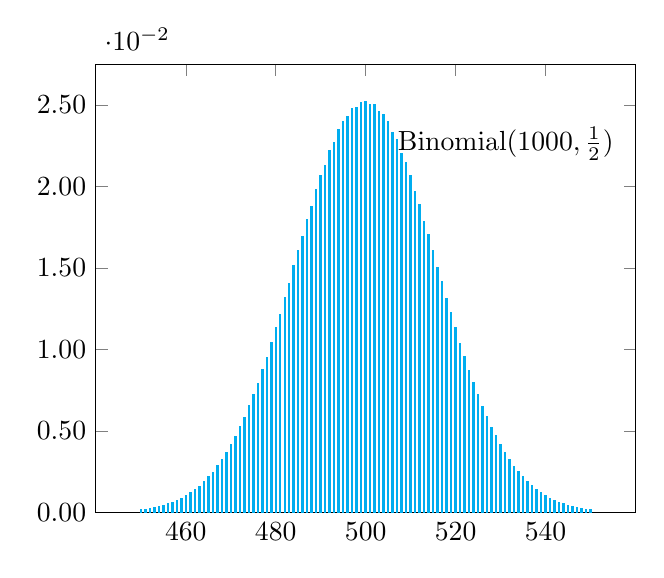
\begin{tikzpicture}
    \begin{axis}
    [
        % Define probability distribution functions
        declare function={
            binom(\n,\p) = \n!/(x!*(\n-x)!)*\p^x*(1-\p)^(\n-x);
            normal(\m,\s) = 1/(\s*sqrt(2*pi))*exp(-((x-\m)^2)/(2*\s^2));
        },
        % Plotting options
        xmin=440, xmax=560,
        ymin=0.0, ymax=0.0275,
        samples at={450,...,550},
        xtick={460,480,...,540},
        ytick={0,0.005,...,0.025},
        yticklabel style={
            /pgf/number format/fixed,
            /pgf/number format/fixed zerofill,
            /pgf/number format/precision=2,
        },   
    ]
    
    % Plot Binomial Distribution
    \addplot [draw=cyan,ybar=0pt,bar width=0.5pt,fill=cyan] {binom(1000,0.5)};
    % Add "discrete CDF" label
    \node[anchor=south west] at (axis cs:505,0.021) {Binomial(\(1000, \frac{1}{2}\))};
    \end{axis}
    \end{tikzpicture}